\section{Метод Эйлера}\label{sec:euler}
Наивное интегрирование методом Эйлера:
\begin{equation}
    \mathbf S_{n+1} = \mathbf S_{n} + h\Delta{\mathbf S_n}
\end{equation}
где $h$ -- скорость в методе Эйлера, а
\begin{equation}
    \Delta{\mathbf S_n} = -|\gamma|\left[\mathbf S_n \times \mathbf H^{eff}\right]
\end{equation}

Относительным временем будем называть величину
\begin{equation}
    \tau = \iota \cdot h
\end{equation}
где $\iota$ номер итерации.
На графике зависимости энергии системы от относительного времени видно
, что метод
Эйлера не применим на допустимых скоростях.
Также не сохраняется длина векторов спинов
И суммой проекций всех спинов на вектор магнитного поля

\begin{figure}[p]
    \centering
    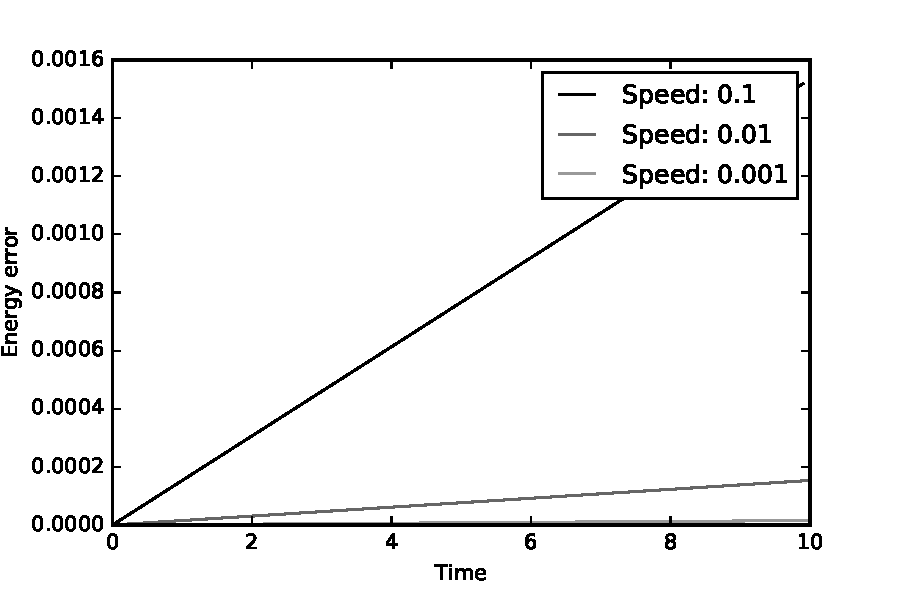
\includegraphics{eulerEnergy.pdf}
    \caption{Зависимость погрешности енергии в методе Эйлера от времени}
\end{figure}
\begin{figure}[p]
    \centering
    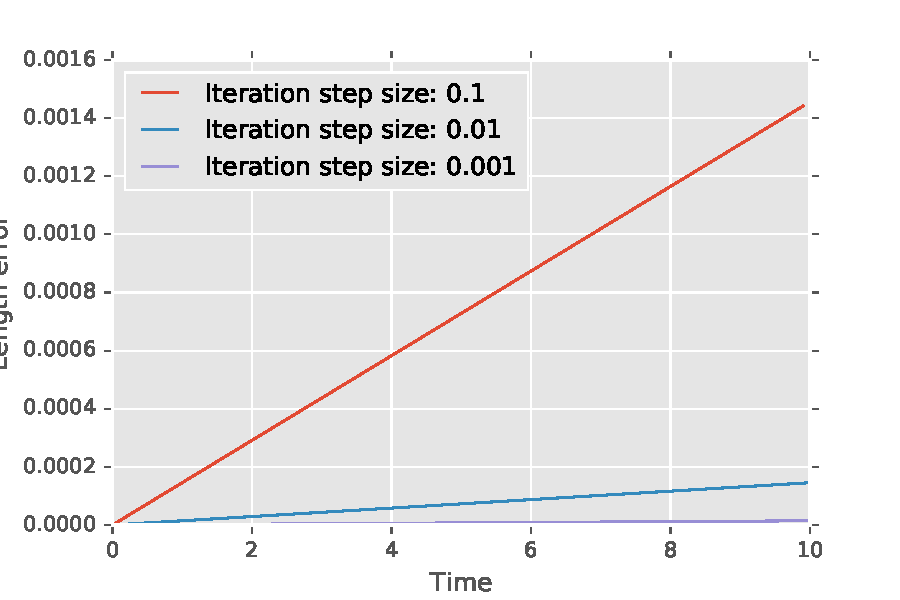
\includegraphics{eulerLength.pdf}
    \caption{Зависимость погрешности суммы длин векторов в методе Эйлера от
    времени}
\end{figure}
\begin{figure}[p]
    \centering
    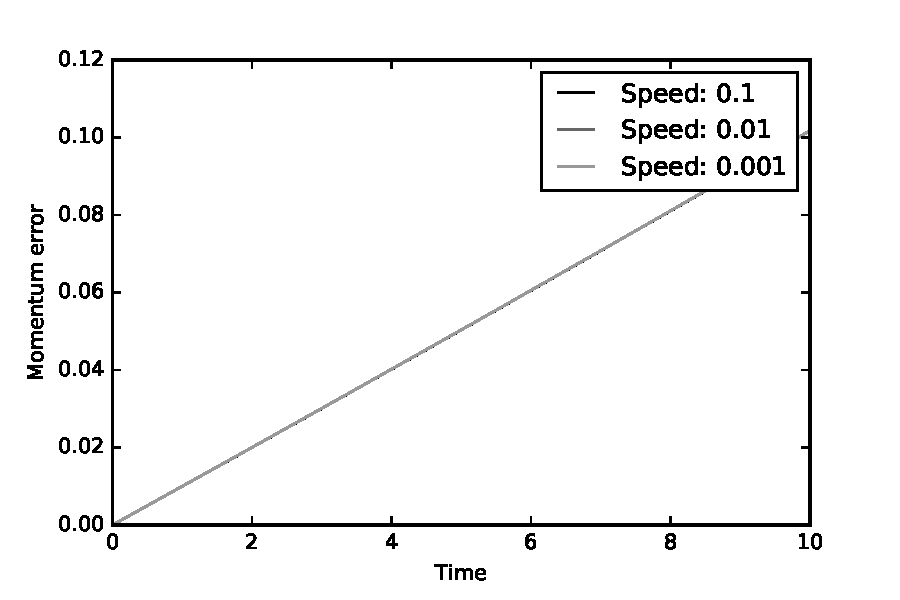
\includegraphics{eulerMomentum.pdf}
    \caption{Зависимость погрешности момента в методе Эйлера от времени}
\end{figure}
\begin{figure}[p]
    \centering
    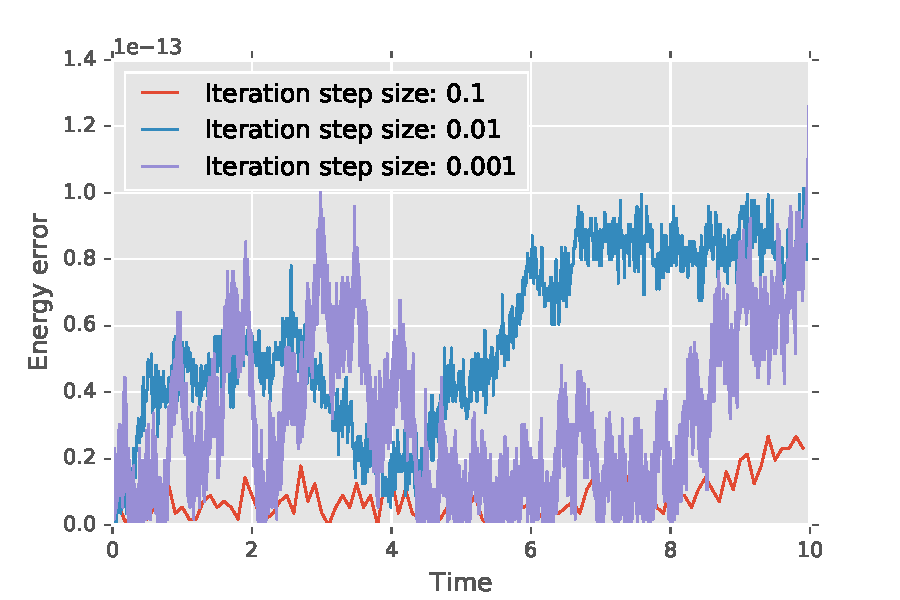
\includegraphics{gauss2Energy.pdf}
    \caption{Зависимость погрешности енергии в методе
    Гаусса-Лежандру-Рунге-Кутта от времени}
\end{figure}
\begin{figure}[p]
    \centering
    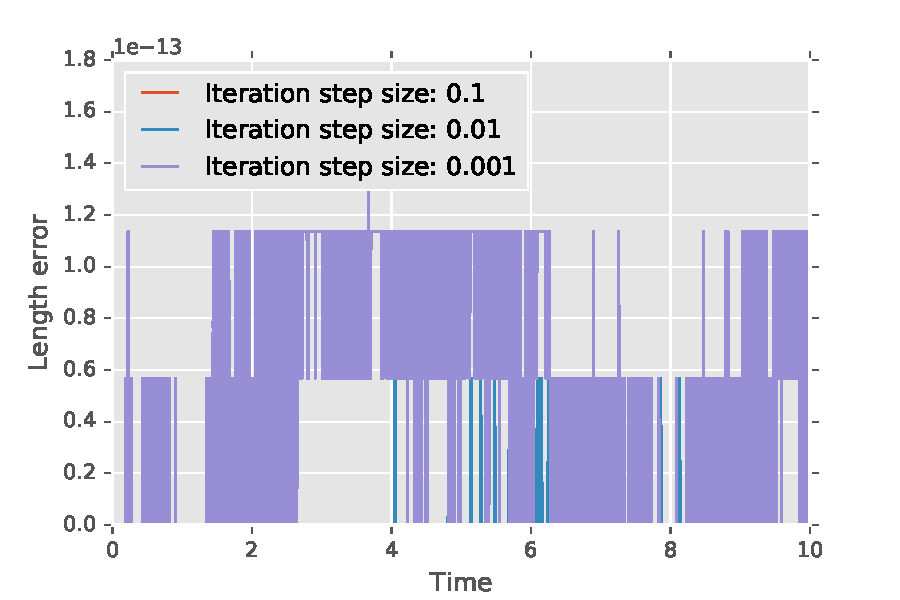
\includegraphics{gauss2Length.pdf}
    \caption{Зависимость погрешности суммы длин векторов в методе
    Гаусса-Лежандру-Рунге-Кутта от времени}
\end{figure}
\begin{figure}[p]
    \centering
    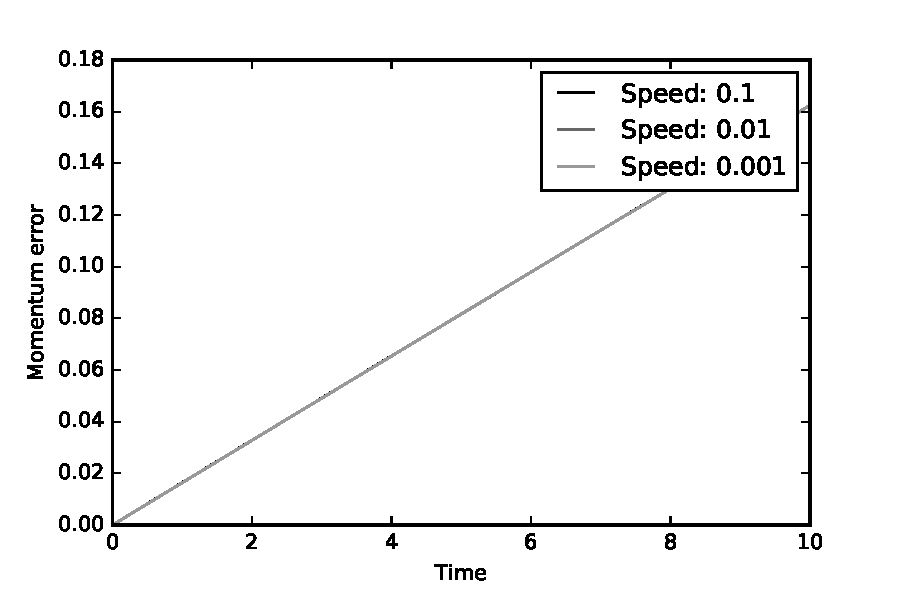
\includegraphics{gauss2Momentum.pdf}
    \caption{Зависимость погрешности енергии в методе
    Гаусса-Лежандру-Рунге-Кутта от времени}
\end{figure}


Для сохранения длины спинов можно на каждой итерации нормировать все вектора из
$\mathbf S$, тогда графики будут выглядеть как  и
 для энергии системы и проекции векторов на
направление магнитного поля соответственно.
